% \documentclass[a4, 12pt]{article}
\documentclass[12pt]{article}
\usepackage[margin=.5cm]{geometry}
\usepackage{amsmath, multicol, amssymb, graphicx, subcaption}
\raggedcolumns

\usepackage{xcolor, titlesec} % For color management

% Set width of the rule (e.g., 0.4pt or thicker)
\setlength{\columnseprule}{0.4pt}

% Set the color of the rule to black
\def\columnseprulecolor{\color{black}}

\titleformat{\section}
  {\normalfont\Large\bfseries} % Font formatting
  {\thesection}{1em} % Label and spacing
  {}[\titlerule] % Draws a line (overline) after the title

%===Borra la identación de forma global===
\setlength{\parindent}{0pt}


% \title{}
% \author{}
\date{}

\begin{document}
    \begin{multicols}{2}
        \section*{Relatividad General}
        \subsection*{Ecuaciones básicas}
        Ecuación de Einstein:
        \begin{equation*}
            G_{\mu\nu} \equiv R_{\mu\nu} - g_{\mu\nu}R = \frac{8 \pi G}{c^4}T_{\mu\nu}
        \end{equation*}

        La condición para métrica \textbf{plana}:
        \begin{equation*}
            R^{\mu}_{\mu\rho\sigma} = 0 \Rightarrow R = 0
        \end{equation*}

        Para $d=2$ y una métrica diagonal:
        \begin{equation*}
            \begin{aligned}
                &ds^2 = f(x,y)dx^2 + h(x, y)dy^2 \\
                &R = \frac{-1}{\sqrt{f\cdot h}}\bigg[ \partial_x \bigg( \frac{\partial_x h}{\sqrt{f\cdot h}}\bigg) + \partial_y \bigg( \frac{\partial_yf}{\sqrt{f \cdot h}} \bigg)\bigg]
            \end{aligned}
        \end{equation*}

        Para un métrica como la mencionada abajo, donde $d$ es la dimensión y $g$ es el \textit{tensor métrico}, vale que:
        \begin{equation*}
            \begin{aligned}
            &ds^{2}_{d+1} = (dx^{d+1})^2 + \Omega(x^{d+1})g_{ij}dx^idx^j \\
            &R_{d+1} = \frac{R_d}{\Omega} -d\frac{\Omega''}{\Omega} - \frac{d(d-3)}{4}\frac{(\Omega')^2}{(\Omega)^2}
            \end{aligned}
        \end{equation*}

        \subsection*{Geodésicas}
        La ecuación de las geodésicas está dada por:
        \begin{equation*}
            \frac{d^2x^\mu}{ds^2} + \Gamma^{\mu}_{\sigma\rho} \frac{dx^{\sigma}}{ds} \frac{dx^{\rho}}{ds} = 0
        \end{equation*}

        Pero otra forma mas práctica es calculando las ecuaciones de \textit{Euler-Lagrange} del siguiente Lagrangeano:
        \begin{equation*}
            \mathcal{L} = g_{\mu\nu} \frac{dx^{\mu}}{d\Lambda} \frac{dx^{\nu}}{d\Lambda}
        \end{equation*}
        
        \section*{Standard Model}
        \begin{equation*}
            \mathcal{L}_{SM} = \mathcal{L}_{Dirac} + \mathcal{L}_{Higgs} + \mathcal{L}_{gauge} + \mathcal{L}_{Yukawa}
        \end{equation*}

        \subsection*{Dirac}
        El $\mathcal{L}_{Dirac}$ está dado por:
        \begin{equation*}
            \mathcal{L}_{Dirac} = \sum_{i=1}^{6} \bar{\Psi}_i i \gamma^{\mu} D_{\mu} \Psi_i
        \end{equation*}

        Términos de interacción con \textbf{interacciones fuertes} (resultan de guagear $SU(3)_{color}$):
        \begin{equation*}
            \sum_{f} g\;\bar{\psi}_{f} \gamma^{\mu} A_{\mu}^a \frac{\lambda_{a}}{2} \psi_f \quad \rightarrow \psi_f = \begin{pmatrix} \psi_{f}^{(R)} \\\psi_{f}^{(G)} \\ \psi_{f}^{(B)} \end{pmatrix}
        \end{equation*}

        Las \textit{electro-débiles} salen de gaugear $U(1)_Y \times SU(2)_L$. Las interacciones con \textbf{$A_{\mu} y Z^{0}$} son:
        \begin{equation*}
            \bar{\Psi}Q\gamma^{\mu}A_{\mu}\Psi + \bar{\Psi}_R \gamma_{\mu}Z_{\mu}C_{R}\Psi_R + \bar{\Psi}_{L}\gamma^{\mu}Z_{\mu}C_{L}\Psi_{L}
        \end{equation*}

        Las interacciones con los bosones $W^{\pm}$:
        \begin{equation*}
            -\frac{1}{\sqrt{2}}\bigg(\bar{\Psi}^{up}_{L} \gamma^{\mu} W_{\mu}^{+} \Psi_{L}^{down} + \bar{\Psi}_{L}^{down}\gamma^{\mu}W_{\mu}^{-}\Psi_{L}^{up}\bigg)
        \end{equation*}

        \subsection*{Higgs}
        \begin{equation*}
            \begin{aligned}
                &\mathcal{L}_{Higgs} = (D_{\mu} \Phi)^{\dagger} (D^{\mu} \Phi) - \lambda \bigg(\Phi^{\dagger} \Phi - \frac{\nu^2}{2} \bigg) \\ 
                &\rightarrow \text{ruptura de simetría:}\; \Phi = \binom{0}{\frac{\nu + h(x)}{\sqrt{2}}}  
            \end{aligned}
        \end{equation*}

        Los términos de masa e interacciones con $W^{\pm}$ y $Z^{0}$:
        \begin{equation*}
            \begin{aligned}
                &\text{Masa:} \; g^2 \frac{\nu^{2}}{4}W^{+}W_{-} + (g^2 + g'^{2})\frac{\nu^{2}}{8}Z_{\mu}Z^{\mu} \\
                &\text{Interacción:} \; \frac{g^2}{4}h^2W^{+}W_{-} + \frac{g^2}{8}h^2Z_{\mu}Z^{\mu} + \frac{g^2\nu}{2}hW^{+}W_{-} + \\
                &\frac{(g^2 +g'^{2})}{4}hZ_{\mu}Z^{\mu}
            \end{aligned}
        \end{equation*}

        \subsection*{Yukawa}
        \begin{equation*}
            \mathcal{L}_{Yukawa} = \sum_{i=1}^{6} = \bar{\Psi}_{L} \Phi \Psi_{R} + \bar{\Psi_{R}} \Phi^{\dagger} \Psi_{L}
        \end{equation*}

        Interacción y masa:
        \begin{equation*}
            \text{Masa:} \; -\frac{g_q \nu}{\sqrt{2}}\bar{\psi}\psi \quad
            \text{Interacción:} \; -\frac{g_q}{\sqrt{2}}h\bar{\psi}\psi
        \end{equation*}

        \subsection*{Gauge}
        \begin{equation*}
            \mathcal{L}_{gauge} = - \frac14 B_{\mu\nu}B^{\mu\nu} - \frac14 G^a_{\mu\nu}G^{\mu\nu}_a - \frac14 W^a_{\mu\nu}W^{\mu\nu}_a
        \end{equation*}

        Genéricamente, la dinámica de los campos está dada por:
        \begin{equation*}
            G_{\mu\nu}^{a} = \partial_{\mu}A_{\nu}^{a} - \partial_{\nu}A_{\mu}^{a} - gA_{\mu}^{b}A_{\nu}^{c}f^{bca}
        \end{equation*}

        Acoplamientos (usando $W_{\mu\nu}^{\pm} \equiv \partial_\mu W_{\nu}^{\pm} - \partial_{\nu}W^{\pm}_{\mu}$):
        \begin{equation*}
            \mathcal{L} = -g(W_{\mu\nu}^{-}W^{+\mu}V^\nu - W_{\mu\nu}^{+}W^{-\mu}V^\nu + Z_{\mu\nu}W^{+\mu}W^{-\nu})
        \end{equation*}
        
        \subsection*{Conservaciones}
        Número léptónico:
        \begin{equation*}
            N_L^{familia} = (N_{\psi_1} - N_{\bar{\psi_1}}) + (N_{\psi_2} - N_{\bar{\psi_2}})
        \end{equation*}

        Número bariónico
        \begin{equation*}
            N_B^{familia} = \frac13 \bigg[(N_{\psi_1} - N_{\bar{\psi_1}}) + (N_{\psi_2} - N_{\bar{\psi_2}})\bigg]
        \end{equation*}

        Carga:
        \begin{equation*}
            \frac{Q_{R|L}}{e} = \frac{Y_{L|R}}{2} + \frac{\sigma_3}{2} \rightarrow Y_L = -id \quad Y_R:diag
        \end{equation*}
        $\sigma_3$ solo para Left

        \section*{Cosas no importantes}
        \textbf{Símbolos de Christoffell}:
        \begin{equation*}
            \Gamma^{\mu}_{\sigma\rho} = \frac{1}{2} g^{\mu\nu} \bigg(\partial_{\rho} g_{\sigma\nu} + \partial_{\sigma} g_{\rho\nu} - \partial_{\nu} g_{\rho\sigma} \bigg)
        \end{equation*}

        \textbf{Regla para las masas}: $\mathbb{C} \rightarrow \mathcal{L}_{masa} = - m^{2} \Phi^{\dagger}\Phi$, $\mathbb{R} \rightarrow \mathcal{L}_{masa} = - \frac12 m^{2} \Phi^{2}$. Y para campos de Dirac: $\mathcal{L}_{masa} = -m \bar{\psi}\psi$.

        \textbf{Ángulos de Weigner}:
        \begin{equation*}
            \begin{cases}
                B_{\mu} &= \cos \theta_{W}A_{\mu} - \sin \theta_{W}Z_{\mu} \\
                W_{\mu}^{3} &= \sin \theta_{W}A_{\mu} + \cos \theta_{W}Z_{\mu}
            \end{cases}
        \end{equation*}

        \textbf{Coeficientes left o right}:
        \begin{equation*}
            \begin{cases}
                C_L = e\bigg(-\tan{(\theta_W)\frac{Y_{L}}{2}} + \cot(\theta_{W})\frac{\sigma_3}{2}\bigg) \\
                C_R = -e\tan(\theta_W)\frac{Y_R}{2}
            \end{cases}
        \end{equation*}

        \textbf{Composición de los $W^{\pm}$}:
        \begin{equation*}
            \begin{cases}
                W_{\mu}^{+} = \frac{1}{\sqrt{2}} (W_{\mu}^{1} - iW_{\mu}^{2}) \\
                W_{\mu}^{-} = \frac{1}{\sqrt{2}} (W_{\mu}^{1} + iW_{\mu}^{2}) \\
            \end{cases}
        \end{equation*}

        \textbf{Ángulos de mezcla}:
        \begin{equation*}
            \begin{cases}
                \cos(\theta_{W}) = \frac{g}{\sqrt{g'^{2} + g^{2}}} \\
                \sin(\theta_{W}) = \frac{g'}{\sqrt{g'^{2} + g^{2}}} \\
            \end{cases}
        \end{equation*}

        \textbf{Transformación de los campos} antes una \textit{gaugeo}:
        \begin{equation*}
            \begin{cases}
                A_{\mu}' = \frac{1}{ig}\Omega D_\mu \Omega^{\dagger} \\
                G_{\mu\nu}' = \Omega G_{\mu\nu} \Omega^{\dagger}
            \end{cases}
        \end{equation*}

        Donde $A_{\mu} = A_{\mu}^{a}\frac{T_a}{2}$ y $G_{\mu\nu} = G_{\mu\nu}^{a}\frac{T_a}{2}$

        \textbf{Ecuaciones de Euler-Lagrange}:
        \begin{equation*}
            \frac{d}{d\Lambda} \bigg( \frac{\partial \mathcal{L}}{\partial (\phi')} \bigg) - \frac{\partial \mathcal{L}}{\partial \phi} = 0 \bigg/ \phi' = \frac{\partial\phi}{\partial \Lambda}
        \end{equation*}

        \textbf{Dimensión del grupo}:
        \begin{equation*}
            \begin{aligned}
                &dim(U(N)) = N^2\\
                &dim(SU(N)) = N^2 - 1
            \end{aligned}
        \end{equation*}

        \textbf{Noether}
        Supongamos $L = L(\phi_1, ..., \phi_N, \partial_\mu \phi_1, ..., \partial_\mu \phi_N)$, aplicando transformación infinitesimal:

        \begin{equation*}
            \begin{split}
                &L' = L + \partial_\mu K^\mu \\ 
                &\Rightarrow J^\mu = \sum_i \frac{\partial L}{\partial(\partial_\mu\phi)} \Delta \phi_i + \partial_\mu K^\mu \\
                &\partial_\mu J^\mu = 0 \quad \text{(Bajo ecs de mto)}
            \end{split}
        \end{equation*}

    \end{multicols}
    Resumen en imágenes:

    \begin{figure}[h!]
        \centering
        \begin{subfigure}[b]{.45\textwidth}
            \centering
            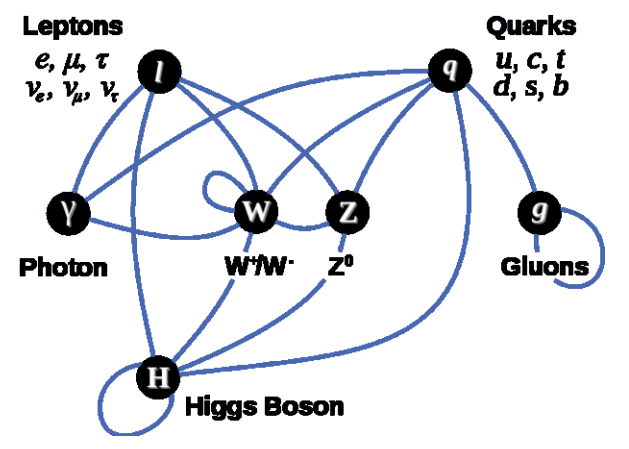
\includegraphics[width=1\textwidth]{src/resumen_SM.png}
        \end{subfigure}
        \hfill % Adds horizontal space between the two images
        \begin{subfigure}[b]{.45\textwidth}
            \centering
            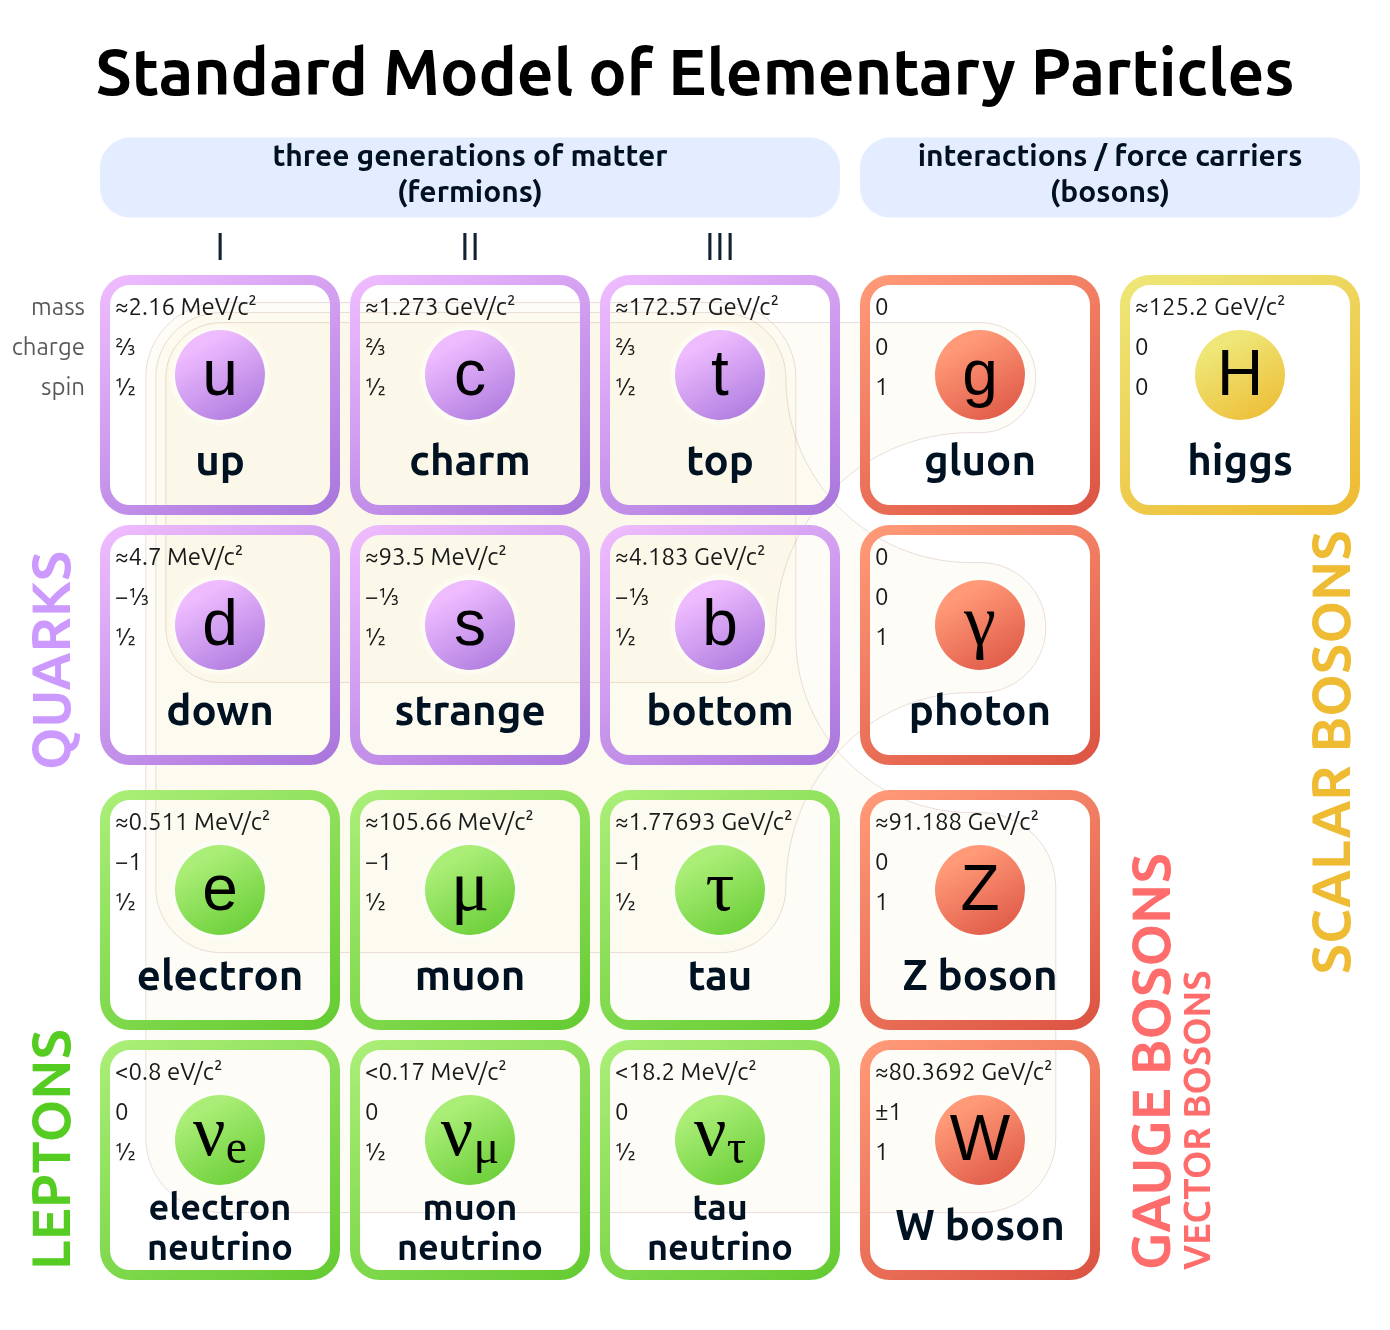
\includegraphics[width=1\textwidth]{src/standard model.png}
        \end{subfigure}
    \end{figure}

\end{document}